%CS 109 Problem Set Xiaoqi Zhou


\documentclass{article}
	% basic article document class
	% use percent signs to make comments to yourself -- they will not show up.

\usepackage{amsmath}
\usepackage{amssymb}
	% packages that allow mathematical formatting

\usepackage{graphicx}
\usepackage{float}
	% package that allows you to include graphics

\usepackage[top=1in, bottom=1in, left=1in, right=1in]{geometry}

\frenchspacing
	% one space after periods

\usepackage{fancyhdr}
	% allows custom headers

\pagestyle{fancy}

\lhead{CS 109, Stanford University \\ Problem Set \#5} 
\rhead{Xiaoqi Zhou (xqzhou@stanford.edu) \\ 06237147}
\usepackage{color}
\usepackage{courier}
\usepackage{relsize}
\usepackage{verbatim}
\cfoot{\thepage}
\renewcommand{\footrulewidth}{0.4pt} 
	%footer
\newcommand{\myansw}{\textbf{Answer:}\\}
\newcommand{\mysolu}{\textbf{Solution:}\\}
\begin{document}
\thispagestyle{fancy} %shows header/footer

\begin{enumerate}
	\item
	%1
	\begin{enumerate}
		\item
		\myansw
		The after trial distribution is:\\
		\colorbox{yellow}{${f(x) = Beta(2+7, 2+2)  = Beta(9,4)}$}\\
		\item
		\myansw
		${F_{Beta}(0.5) = 0.073}$\\
		\colorbox{yellow}{${P(\text{drug having effect} \geq 0.5) = 1 - F_{Beta}(0.5) = 0.927}$}\\
		
	
		
	\end{enumerate}
	\item
	\begin{enumerate}
		\item
		\myansw
		${P(35 \leq X \leq 40) = 0.00022}$\\
		${P(40 \leq X \leq 45) = 0.04192}$\\
		${P(60 \leq X \leq 65) = 0.00022}$\\
		
		\begin{figure}[H]
			\centering
			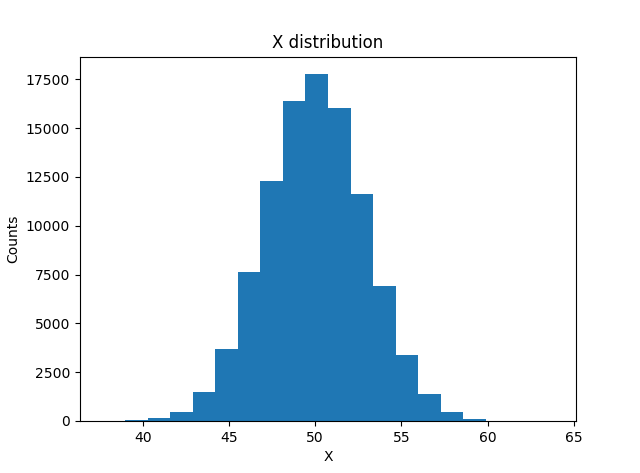
\includegraphics[width=0.8\textwidth]{pset_5_2_a.png}
		\end{figure}
		\item
		\mysolu
		From the simulation results, we can find\\
		${E[X] = 50.00}$\\
		${Var(X) = 8.336}$\\
		Then we can use normal distribution to represent the distribution.\\
		\myansw
		\colorbox{yellow}{${X \sim N(50.00, 8.336)}$}\\
		\colorbox{yellow}{${f(x) = \frac{1}{\sqrt{2\pi8.336}}e^{-(x-50)^2/(2\times 8.336)}}$}\\
		\item
		\mysolu
		${P\{40 \leq X \leq 45\}= F(45) - F(40) =\Phi(\frac{(45 -50)}{\sqrt{8.336}}) -  \Phi(\frac{(40 -50)}{\sqrt{8.336}})}$\\
		\colorbox{yellow}{text${P\{40 \leq X \leq 45\}= \Phi(\frac{10}{2.89}) -  \Phi(\frac{5}{2.89}) = 0.9997 - 0.9582 = 0.0415}$}\\
		
		
		
	\end{enumerate}
	\item
	\begin{enumerate}
	\item
		\myansw
		The expected amount of money that each person gives is\\
		\colorbox{yellow}{${E[X] = 5.95}$}\\
		\item
		\myansw
		\colorbox{yellow}{${Var(X) = E[X^2]-(E[X])^2 = 23.55}$}\\
		\item
		\mysolu
		${E[n\overline{X}]= nE[X]= 5.95 \times 50 =297.5}$\\
		${Var(n\overline{X}) = nVar(X)=1159.5}$\\
		\myansw
		\colorbox{yellow}{${\sum\limits_{i = 1}^{50}X_i \sim N(297.5, 1177.5)}$}\\		
		\item
		\myansw
		${Y = \sum\limits_{i = 1}^{50}X_i}$\\
		\colorbox{yellow}{${P\{Y \geq 350\} = 1 - P\{Y < 350\} = 1 - \Phi(\frac{350 - 297.5}{\sqrt{1177.5}}) = 1 - 0.9370  = 0.063}$}
		

	\end{enumerate}
	\item
	\mysolu 
	${Cov(X,Y) = Cov(X,X^2) = E[X^3] - E[X]E[X^2]}$\\
	$E[X^3] = \frac{1}{6}\sum\limits_{i = 1}^{6}i^3 = 73.5$\\
	$E[X^2] = \frac{1}{6}\sum\limits_{i = 1}^{6}i^2 = 15.17$\\
	$E[X] =\frac{1}{6}\sum\limits_{i = 1}^{6}i = 3.5 $\\
	\myansw
	\colorbox{yellow}{${Cov(X,Y) = 20.41}$}\\
	
	\item 
	\myansw
	\colorbox{yellow}{${2X + Y \sim N(2+1, 2\times 4 + 2)}$}\\
	\colorbox{yellow}{${2X + Y \sim N(3, 10)}$}\\
	\item
	\begin{enumerate}
		\item 
		\myansw
		Let X be the true distance of the satellite\\
		\colorbox{yellow}{$f_X(x) = \frac{1}{4\sqrt{2\pi}}e^{-(x-98)^2/32}$}\\
		\item
		\myansw
		Let Y be the measured distance\\
		\colorbox{yellow}{$f_{Y|X}(y = 100|x = t) = \frac{1}{2\sqrt{2\pi}}e^{-(100-t)^2/8}$}\\
		\item
		\mysolu
		Let X' be the posterior belief of the true distance of satellite\\
		$f_{XY}(x, y = 100) =f_{Y|X}(y = 100|x )f_X(x)=\frac{1}{2\sqrt{2\pi}}e^{-(100-x)^2/8}\times \frac{1}{4\sqrt{2\pi}}e^{-(x-98)^2/32} $\\
		$\mathlarger{f_{X'}(x') = f_{X|Y}(x=x' | y = 100) = \frac{f_{XY}(y = 100, x=x')}{f_Y(y = 100)} = \frac{f_{XY}(x=x',y = 100)}{\mathlarger{\int_{-\infty}^{+\infty}f_{XY}(y = 100)dx}}}$\\
		Let\\
		$\mathlarger{C = \frac{1}{\mathlarger{\int_{-\infty}^{+\infty}f_{XY}(x,y = 100)dx}}}$\\
		\myansw
		\colorbox{yellow}{$\mathlarger{f_{X'}(x') = C\frac{1}{16\pi^2}e^{\frac{-(4(100-x')^2+(x'-98)^2)}{32}}}$}\\
	\end{enumerate}
	\item
	\begin{enumerate}
		\item
		\mysolu
		Let $X_n$ be the total value of the $n$th rolling before any value $\geq$ 3 is rolled\\
		$E[X] = \sum\limits_{i = 0}^{\infty}E[X_i]+4.5$\\
		Let $Y$ be the value when for each rolling when value $<$ 3\\
		$E[Z] = 1.5$\\
		$E[X_i] = (\frac{1}{3})^i(E[Z]) = 1.5(\frac{1}{3})^i$\\
		\myansw
		\colorbox{yellow}{$E[X] = \sum\limits_{i = 1}^{\infty} 1.5(\frac{1}{3})^i+4.5 = 1.5\frac{\frac{1}{3}}{(1-\frac{1}{3})}+4.5=5.25$}\\
		\item
		\myansw
		\colorbox{yellow}{$E[Y] = \sum\limits_{i = 1}^{\infty} (\frac{1}{3})^i+1 = \frac{\frac{1}{3}}{(1-\frac{1}{3})}+1=1.5$}\\		
		
		
	\end{enumerate}
	\item
	\mysolu
	$E[Y^2] = E[Y^2|X = 1]P(X = 1)+E[Y^2|X = 2]P(X = 2)+E[Y^2|X = 2]P(X = 2)$\\
	$E[Y^2] = E[3^2]\frac{1}{3}+E[(Y+5)^2]\frac{1}{3}+E[(Y+7)^2]\frac{1}{3}$\\
	$3E[Y^2] = 9+E[Y^2]+10E[Y]+25 + E[Y^2]+14E[Y]+49$\\
	$E[Y^2] = 443$\\
	\myansw
	\colorbox{yellow}{$Var(Y) = E[Y^2]-E[Y]^2 = 443 - 225 = 218$}\\
	\item
	\begin{enumerate}
		\item
		\mysolu
		$E[n\overline{A}] = n\mu_A = 20 \times 50 = 1000$\\
		$Var(n\overline{A}) = n^2\frac{\sigma_A^2}{n} = n\sigma_A^2 = 2000$\\
		$P(n\overline{A} < 950) = \Phi(\frac{950 - 1000}{\sqrt{2000}}) = 1 - \Phi(\frac{50}{44.72})= 1- 0.8686$\\
		\colorbox{yellow}{$P(n\overline{A} < 950)= 0.1314$}\\
		\item 
		$E[n\overline{B}] = n\mu_B = 20 \times 52 = 1040$\\
		$Var(n\overline{B}) = n^2\frac{\sigma_B^2}{n} = n\sigma_B^2 = 4000$\\
		$P(n\overline{B} < 950) = \Phi(\frac{950 - 1040}{\sqrt{4000}}) = 1 - \Phi(\frac{90}{44.72})= 1- 0.9207$\\
		\colorbox{yellow}{$P(n\overline{B} < 950)= 0.0793$}\\
		\item
		Let $C = A - B$\\
		$E[n\overline{C}] = n\mu_C= \mu_A - \mu_B = -40 $\\
		$Var(n\overline{C}) = n\sigma_C^2 = n(\sigma_A^2 + \sigma_B^2) = 6000$\\
		\myansw
		\colorbox{yellow}{$P(C < 0) = F_C(0) = \Phi(\frac{0-(-40)}{\sqrt{6000}})=0.6985$}\\
	\end{enumerate}
	\item
	\mysolu
	Let $Y = \sum\limits_{i = 1}^{79}X_i$\\
	$E[Y] = 79E[X] = 79\times3.5 = 276.5 $\\
	$Var(Y) = 79Var(X)  $\\
	$Var(X) = E[X^2] - E[X]^2 = 2.92$\\
	$Var(Y) = 230.68$\\
	$Y \sim N(276.5, 230.68)$\\
	When the first 79 rolls have sum lower than 300, at least 80 rolls are necessary to reach a sum that exceeds 300.\\
	$P(Y \leq 299.5) = F_Y(299.5)  = \Phi(\frac{299.5 - 276.5}{sqrt{230.68}})$\\
	\myansw
	\colorbox{yellow}{$P(Y \leq 299.5) = 0.9332$}\\
	
	
	\item
	\begin{enumerate}
		\item
		\myansw 
		\colorbox{yellow}{$P(X \geq 85) \leq \frac{E[X]}{85} = 0.882$}\\
		\item 
		\mysolu
		$P (65 \leq X \leq 85) > P(|X - 75|< 10) = 1 - P(|X - 75|\geq 10)$\\
		$P(|X - 75| \geq 10) \leq \frac{Var(X)}{10^2} = 0.25$\\
		$0.75 \leq 1 - P(|X - 75|\geq 10)< P (65 \leq X \leq 85) $\\
		\myansw
		\colorbox{yellow}{$ P (65 \leq X \leq 85) > 0.75$}\\
		\item
		\mysolu
		Let $Y = \overline{X}$\\
		$E[Y] = E[X] = 75$\\
		$Var(Y) = \frac{Var(X)}{n} = \frac{25}{n}$
		$P(|Y - 75| \geq 5) \leq \frac{Var(Y)}{5^2} = \frac{\frac{25}{n}}{25}\leq 0.1$\\
		\myansw
		$\frac{1}{n}\leq 0.1$\\
		The number of students would have to take the midterm in order to ensure 90\% probability that the class average would be within 5 of 75 is\\
		\colorbox{yellow}{$n \geq 10$}\\
		\item
		\mysolu
		$P(-5 \leq \overline{X} - E[X] \leq 5) = \Phi(\frac{5}{\frac{\sigma}{\sqrt{n}}})-\Phi(\frac{-5}{\frac{\sigma}{\sqrt{n}}})= 2\Phi(\frac{5}{\frac{5}{\sqrt{n}}}) - 1 \geq 0.9$\\
		$\Phi(\sqrt{n})>0.95$
		$\sqrt{n}>1.65$\\
		\myansw
		The number of students would have to take the midterm in order to ensure 90\% probability that the class average would be within 5 of 75 is\\
		\colorbox{yellow}{$n =3>2.72 $}\\
		
		
		
	\end{enumerate}
	\item
	\begin{enumerate}
		\item
		\myansw
		\colorbox{yellow}{$P(S = true|G = female, C= 1) = 0.968$}\\
		\colorbox{yellow}{$P(S = true|G = female, C= 1) = 0.921$}\\
		\colorbox{yellow}{$P(S = true|G = female, C= 1) = 0.5$}\\
		\colorbox{yellow}{$P(S = true|G = female, C= 1) = 0.369$}\\
		\colorbox{yellow}{$P(S = true|G = female, C= 1) = 0.157$}\\
		\colorbox{yellow}{$P(S = true|G = female, C= 1) = 0.137$}\\
		\item
		\mysolu
		Total third class children is 53, and 22 of them survived.\\
		We can use the conditional of all the third class passengers as a prior distribution\\
		Total third class passenger number is 487, 119 of them survived\\
		Let\\
		$a = 487 + 1 = 488$\\
		$b = 119 + 1 = 120$\\
		$m = 22$\\
		$n = 31$\\
		\myansw
		$S \sim Beta(a+m, b+n)$\\
		\colorbox{yellow}{$S \sim Beta(510, 151)$}\\
		\item
		\myansw
		\colorbox{yellow}{$E[X|C=1]= 84.15$}\\
		\colorbox{yellow}{$E[X|C=1]= 20.66$}\\
		\colorbox{yellow}{$E[X|C=1]= 13.71$}\\

		
	\end{enumerate}
	\item
	\begin{enumerate}
		\item
		\myansw
		\colorbox{yellow}{$\overline{X} = 69.22$}\\
		\item
		\mysolu
		$Y = \overline{X}$\\
		$S^2 = \sum\limits_{i = 1}^{n}\frac{(Y_i - \overline{Y})}{n-1}$\\
		
		\textbf{Code:}\\
		\begin{verbatim}
		n = 100000 #repeat 100000 loops
		grade_mean_array = numpy.zeros(n)
		index = [0]*5
		for i in range(0,n):
		    for j in range(0,5):
		        #Generate 5 random index for each grades
		        index[j] = int(numpy.floor(numpy.random.rand()*10000))
		    grade_mean_array[i] = numpy.mean(grade_array[index])#Get mean of the 5 grades
		#Calculate the expectation of all the mean values
		grade_mean_expectation = numpy.mean(grade_mean_array)
		grade_mean_s = float(0)
		for i in range(0, len(grade_mean_array)):
		    grade_mean_s = grade_mean_s \
		                    + ((grade_mean_array[i] - grade_mean_expectation)**2)\
			                /(len(grade_mean_array)-1) #Calculate S^2 


		print("grade mean expectation: %f"%(grade_mean_expectation))
		print("grade mean variance: %f"%(grade_mean_s))	
		

		\end{verbatim}

		\myansw
		$E[Y] = 69.22$\\
		\colorbox{yellow}{$S^2=101.18$}\\
		\item
		\mysolu
		$Z = median(X)$\\
		$S^2 = \sum\limits_{i = 1}^{n}\frac{(Z_i - \overline{Z})}{n-1}$\\
		
		\textbf{Code:}\\
		\begin{verbatim}
		n = 100000 #repeat 100000 loops
		grade_median_array = numpy.zeros(n)
		index = [0]*5
		for i in range(0,n):
		    for j in range(0,5):
		        # Generate 5 random index for each grades
		        index[j] = int(numpy.floor(numpy.random.rand()*10000))
		    # Get median of the 5 grades
		grade_median_array[i] = numpy.median(grade_array[index])
		#Calculate the expectation of all the median values
		grade_median_expectation = numpy.mean(grade_median_array)

		grade_median_s = float(0)
		for i in range(0, len(grade_median_array)):
		    grade_median_s = grade_median_s \
		                     + ((grade_median_array[i] - grade_median_expectation)**2)\
		                     /(len(grade_median_array)-1) #Calculate S^2


		print("grade mean expectation: %f"%(grade_median_expectation))
		print("grade mean variance: %f"%(grade_median_s))
		
		
		\end{verbatim}
		
		\myansw
		$E[Z] = 73.60$\\
		\colorbox{yellow}{$S^2=56.04$}\\
		\item
		\myansw
		$E[Y] = 69.22$\\
		$E[Z] = 73.60$\\
		\colorbox{yellow}{The expected median of 5 grades is different than the expected mean of 5 grades.}\\
		\item
		\mysolu
		\begin{figure}[H]
			\centering
			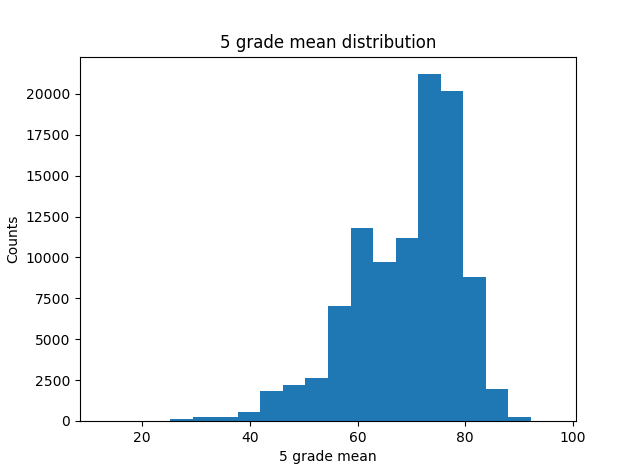
\includegraphics[width=0.8\textwidth]{pset_5_13_e_1.png}
		\end{figure}
		\begin{figure}[H]
			\centering
			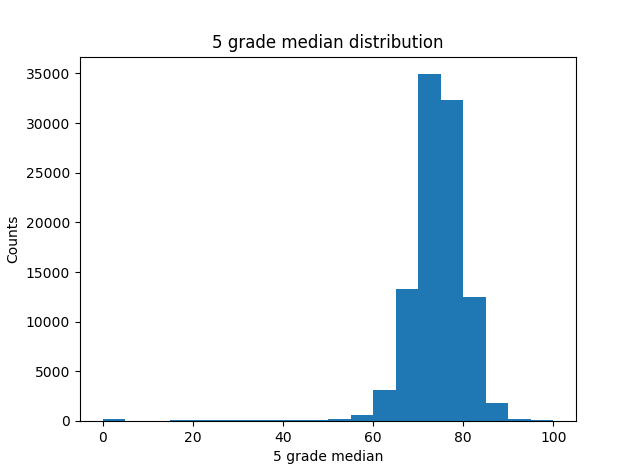
\includegraphics[width=0.8\textwidth]{pset_5_13_e_2.png}
		\end{figure}
		\myansw
		\colorbox{yellow}{Using median of 5 grades is a better way to assign scores,} because the distribution is more like a normal distribution
		
	\end{enumerate}
	\item
	\begin{enumerate}
		\item
		\myansw
		The outcome of activity2 is not independent to activity1. All the student have already learned activity1 when learned activity2. It is difficult to justify outcome of activity2 separately.\\
		\item
		\myansw
		The outcome may not only depend on different activities but also the geographic distribution of the students. The result will be biased by different between the students from eastern vs. western hemisphere.\\
	\end{enumerate}
	\item
	\begin{enumerate}
		\item 
		Let X be the outcome of activity1; Y be the outcome of activity2\\
		$E[X] =144.93 $\\
		$E[Y] = 153.13$\\
		\myansw
		\colorbox{yellow}{$|E[X]-E[Y]| = 8.2$}\\
		\item
		\textbf{Code:}\\
		\begin{verbatim}
		n = 100000 #repeat 100000 times bootstraping
		new_diff = numpy.zeros(n)
		p_num = float(0)
		for i in range(0,n):
		    #select same size of activity1 from uniform dataset
		    new_selection_1 = numpy.array(random.sample(outcome, int(num_1)))
		    #select same size of activity2 from uniform dataset
		    new_selection_2 = numpy.array(random.sample(outcome, int(num_2)))
		    #calculate mean of new activity1
		    new_mean_1 = numpy.mean(new_selection_1)
		    #calculate mean of new activity2
		    new_mean_2 = numpy.mean(new_selection_2)
		    new_diff[i] = abs(new_mean_1 - new_mean_2)
		    #Compare the new observed difference with the pre-calculated difference
		    if new_diff[i] >= diff:
		        p_num = p_num + 1
		#Calculate P-Value
		p_value = p_num/n
		print("P-Value = %f"%(p_value))
		\end{verbatim}
		\myansw
		\colorbox{yellow}{$P-Value = 0.00478$}\\
		\item
		\mysolu
		We can just separate all the students data into 3 groups first based on the background category (link two .csv file by using first column number). Then calculate the mean difference and p-values.\\
		\myansw
		For "more" experience group\\
		\colorbox{yellow}{$|E[X]-E[Y]| = 28.42$}\\
		\colorbox{yellow}{$P-Value = 0.0000$}\\
		For "average" experience group\\
		\colorbox{yellow}{$|E[X]-E[Y]| = 24.98$}\\
		\colorbox{yellow}{$P-Value = 0.00005$}\\
		For "less" experience group\\
		\colorbox{yellow}{$|E[X]-E[Y]| = 26.02$}\\
		\colorbox{yellow}{$P-Value = 0.0000$}\\
		From the Result we can find that the difference of 2 activities are more significant if we separate the students in different catagory. That means the activities have different outcome distribution in different catagory groups. Mixing the data from all 3 group will lead us to a biased result.
	\end{enumerate}
	
	
\end{enumerate}


\newpage



\end{document}